\section{连接杆零件图制作}\label{sec:lianjieganshitu}
\subsection{生成主视图}
\begin{procedure}
\item 保存连接杆三维模型副本

将构建好的连接杆三维模型另存为“连接杆视图布局.dwg”。

\item 切换至图纸空间

点击命令窗口上面的【布局1】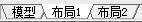
\includegraphics[scale=0.6]{bujukongjian.png} 标签,进入图纸空间。

\item 修改页面设置

调用页面设置管理器,弹出页面设置对话框,将打印机绘图设备修改为“DWG TO PDF.pc3”,图纸尺寸设置为ISO A4(210.00x297.00毫米),设置结果如图\ref{fig:lianjieganpagesetup} 所示。完成后单击图\ref{fig:lianjieganpagesetup}中打印机绘图设备旁边的特性按钮,弹出图\ref{fig:huituyishezhi}所示的绘图仪配置编辑器,选择“设备和文档设置”选项卡中的“修改标准图纸尺寸(可打印区域)”列表,在“修改标准图纸尺寸”对话框中选中ISO A4(210x297毫米),然后点击修改按钮,弹出\ref{fig:kedayinqushezhi}所示可打印区域设置对话框,并按表\ref{tab:tuzhifumian}尺寸设置可打印区域的值。完成设置后,图纸的幅面和可打印区域均符合图家制图的标准要求。

\begin{figure}[htbp]
\centering
\begin{floatrow}[3]
\ffigbox{\caption{面页设置}\label{fig:lianjieganpagesetup}}{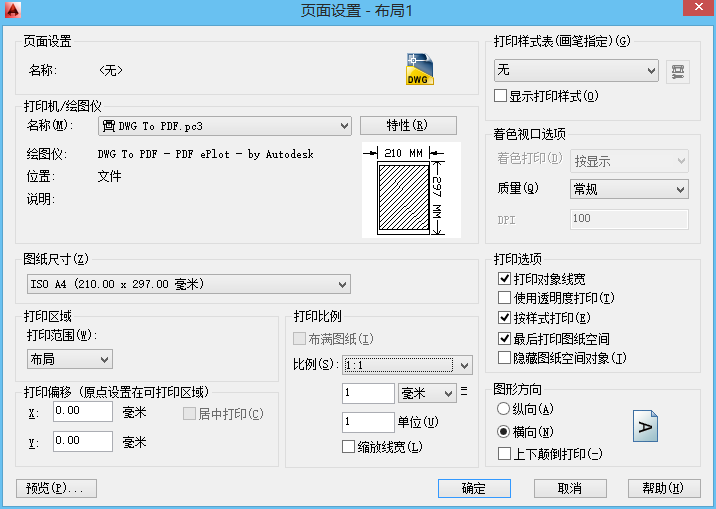
\includegraphics[scale=0.2]{pagesetupdetail.png}}
\ffigbox{\caption{绘图仪配置编辑器}\label{fig:huituyishezhi}}{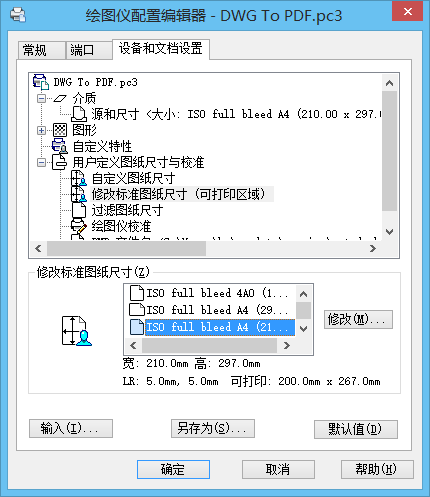
\includegraphics[scale=0.2]{huituyishezhi.png}}
\ffigbox{\caption{可打印区域设置}\label{fig:kedayinqushezhi}}{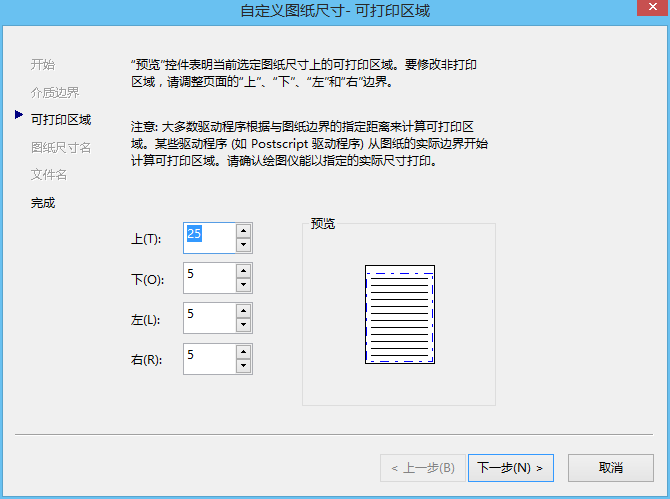
\includegraphics[scale=0.2]{kedayinqushezhi.png}}
\end{floatrow}
\end{figure}

\begin{lstlisting}
命令:pagesetup
\end{lstlisting}

\item 调整图纸空间的连接杆显示设置

首先,进入图纸空间中视口的模型空间。
\begin{lstlisting}
命令:mspace
\end{lstlisting}

其次,将视图方向切换为前视图方向。
\begin{lstlisting}
命令: -VIEW
输入选项 [?/删除(D)/正交(O)/恢复(R)/保存(S)/设置(E)/窗口(W)]: front
\end{lstlisting}
最后,将视口的显示比例设置为2:1,结果如图\ref{fig:lianjiegantuzhi1}所示。
\begin{figure}[htbp]
\centering
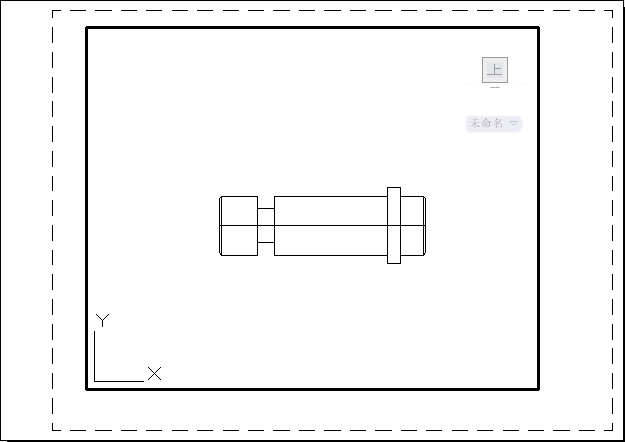
\includegraphics[scale=0.5]{lianjiegantuzhi1.png}
\caption{主视图显设置结果}\label{fig:lianjiegantuzhi1}
\end{figure}
\item 提取视图轮廓,并退出视口模型空间

调用轮廓命令提取视图的轮廓。
\begin{lstlisting}
命令: solprof
选择对象: 找到 1 个
选择对象:
是否在单独的图层中显示隐藏的轮廓线?[是(Y)/否(N)] <是>:
是否将轮廓线投影到平面?[是(Y)/否(N)] <是>:
是否删除相切的边? [是(Y)/否(N)] <是>:
\end{lstlisting}
接下来,退出视口模型空间
\begin{lstlisting}
命令: PSPACE
\end{lstlisting}
\item 修改图层设置

为保证显示正确的主视图,并方便尺寸标注和标题栏的绘制,需要调用图层管理器对图层做设置做以下修改。

\begin{enumerate}
\item 点击新建图层
\includegraphics[scale=0.6]{newlayer.png}图标,新建“标题栏”、“中心线”、“图框”和“尺寸标注”四个新图层。
\item 点击
\includegraphics[scale=0.6]{linewidthselect.png}图标,将PV形状的图层和图框图层的线宽设置为0.5mm。
\item 点击“中心线”图层的线型设置图标
\includegraphics[scale=0.6]{linetypeselect.png},弹出图\ref{fig:linetypeset}所示的选择线型对话框,点击加载按钮,弹出图\ref{fig:loadlinetype}所示的加载或重载线型对话框,然后选择列表框中的CENTER线型并点击确定,返回选择线型对话框中,将CENTER线型选中,如图\ref{fig:selectcenterline}所示。最点击确定完成线型选择。
\item 将中心线图层设置为当前图层。
\end{enumerate}
\begin{lstlisting}
命令:layer
\end{lstlisting}
\begin{figure}[htbp]
\centering
\subfloat[]{\label{fig:linetypeset}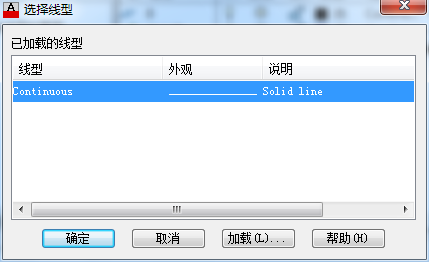
\includegraphics[scale=0.3]{linetypeset.png}}\hspace{20pt}
\subfloat[]{\label{fig:loadlinetype}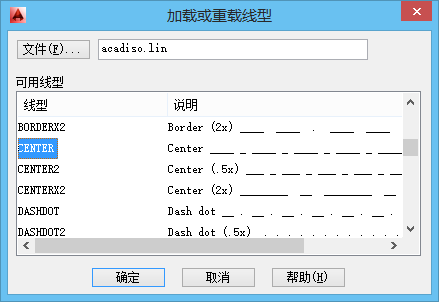
\includegraphics[scale=0.25]{loadlinetype.png}}\hspace{20pt}
\subfloat[]{\label{fig:selectcenterline}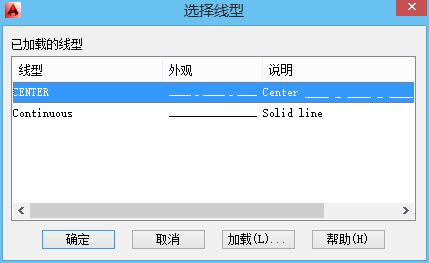
\includegraphics[scale=0.3]{selectcenterline.png}}
\caption{线型设置}
\end{figure}

修改改完成后的图层设置如图\ref{fig:lianjieganlayerset} 所示。
\begin{figure}[htbp]
\centering
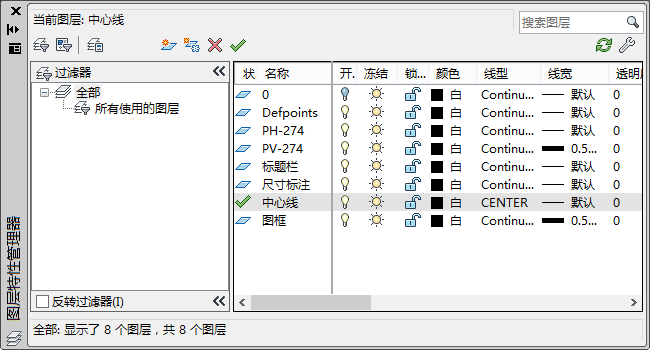
\includegraphics[scale=0.6]{lianjieganlayerset.png}
\caption{连接杆布局图层修改结果}\label{fig:lianjieganlayerset}
\end{figure}
\item 绘制中心线

由于连接杆是对称图形,视图生成后需要在图纸空间中手工绘制一条中线。因此在中心线图层设置为当前的状态下,可用直线命令来完成。AutoCAD中调用直线命令的方式有:
\begin{itemize}
\item 键盘输入line\index{line,直线} 或L。
\item 【绘图】$\rightarrow$【直线】。
\item 【绘图】$\triangleright$【直线】图标
\includegraphics[scale=0.5]{linetool.png}。
\end{itemize}

\begin{figure}[htbp]
\centering
\subfloat[]{\label{fig:centerlinedraw1}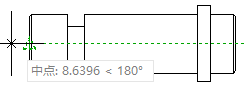
\includegraphics[scale=0.6]{centerlinedraw1.png}}\hspace{20pt}
\subfloat[]{\label{fig:centerlinedraw2}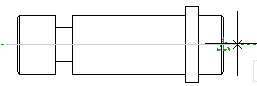
\includegraphics[scale=0.6]{centerlinedraw2.png}}\hspace{20pt}
\subfloat[]{\label{fig:centerlinedraw3}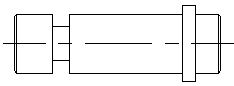
\includegraphics[scale=0.6]{centerlinedraw3.png}}
\caption{绘制中心线}
\end{figure}

\begin{lstlisting}
命令: line
指定第一个点:
\end{lstlisting}
调用直线命令后,命令示示指定第一个点,此时为保证中心线正好绘制在视图的中心,故采用对象捕捉追踪功能来完成第一点的指定,即先用鼠标捕捉到左端线的中心点,然后向左水平移动一小段距离单击鼠标左键指定第一点,如图\ref{fig:centerlinedraw1}所示。
\begin{lstlisting}
指定下一点或 [放弃(U)]:
\end{lstlisting}
命令提示指定下一点时,以指定第一点相同的方式绘定第二点,如图\ref{fig:centerlinedraw2}所示。
\begin{lstlisting}
指定下一点或 [放弃(U)]:
\end{lstlisting}
由于直线命令可以绘制多段直线,因此会继续提示指定下一点,此时用回车键结束命令,结果如图\ref{fig:centerlinedraw3}所示。
\end{procedure}
\subsection{制作图幅}
\begin{procedure}
\item 将当前图层设置为图框
切换图层除了用图层设置管理器,还可以用图层管理工具栏。其方法是点击图层管理工具栏
\includegraphics[scale=0.45]{changelayertools.png}中的图层下拉列表框
\includegraphics[scale=0.5]{changelayers.png},弹出图\ref{fig:changelayers1}的图层列表,并选中图框图层,即可将图框图层设置为当前图层。
\begin{figure}[htbp]
\centering
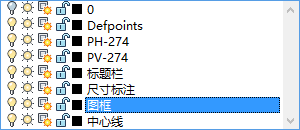
\includegraphics[scale=1]{changelayers1.png}
\caption{图层列表}\label{fig:changelayers1}
\end{figure}
\item 绘制图框

根据A4横向带装订边图幅的尺寸,计算可以得出外图框矩形的尺寸为$267\times 200$,其绘制结果如图\ref{fig:tufukuan1} 所示。
\begin{lstlisting}
命令: RECTANG
指定第一个角点或 [倒角(C)/标高(E)/圆角(F)/厚度(T)/宽度(W)]: 0,0
指定另一个角点或 [面积(A)/尺寸(D)/旋转(R)]: 267,200
\end{lstlisting}

接下来绘制标题的图框,根据标题的尺寸可知其图矩形尺寸为$180\times 56$,其绘制结果如图\ref{fig:tufukuan2} 所示。
\begin{lstlisting}
命令: RECTANG
指定第一个角点或 [倒角(C)/标高(E)/圆角(F)/厚度(T)/宽度(W)]:
指定另一个角点或 [面积(A)/尺寸(D)/旋转(R)]: @-180,56
\end{lstlisting}
\begin{figure}[htbp]
\subfloat[]{\label{fig:tufukuan1}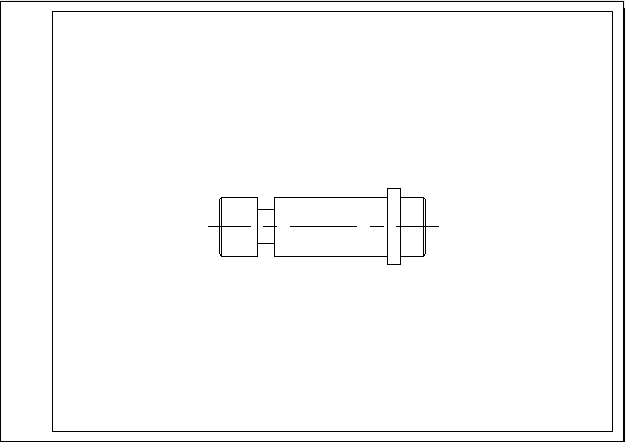
\includegraphics[scale=0.4]{tufukuan1.png}}\hspace{20pt}
\subfloat[]{\label{fig:tufukuan2}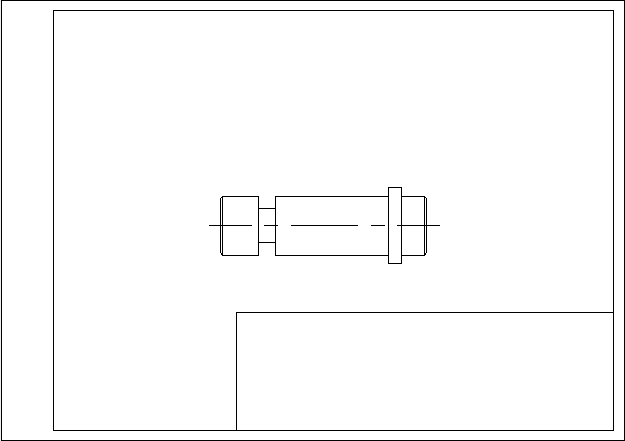
\includegraphics[scale=0.4]{tufukuan2.png}}
\caption{绘制图框}
\end{figure}
\end{procedure}
\subsection{制作标题栏}

根据国家制图标准规定标题栏是每张图样都必须绘制的,且必须位于图样的左下角,其格式和尺寸要遵守国标GB/T10609.1-1989的规定,如图\ref{fig:biaotilan}所示。
\tikzset{
>=latex,
center lines/.style={dash pattern=on 20pt off 3pt on 2pt off 3pt},
importance lines/.style={line width=1pt}
}
\begin{figure}[htbp]
\begin{tikzpicture}[scale=0.65]
\draw[line width=0.7mm](0,0)rectangle(180mm,56mm);
\draw(0,7mm)--(12mm,7mm)--(40mm,7mm)--++(40mm,0);
\draw(6mm,3.5mm)node{\tiny 工艺};
\draw(46mm,3.5mm)node{\tiny 批准};
\draw(0,14mm)--++(80mm,0);
\draw(6mm,10.5mm)node{\tiny 审核};
\draw(0,21mm)--++(12mm,0)--++(12mm,0)--++(16mm,0)--++(12mm,0)--++(12mm,0)--++(16mm,0);
\draw(6mm,24.5mm)node{\tiny 设计};
\draw(18mm,24.5mm)node{\tiny(签名)};
\draw(32mm,24.5mm)node{\tiny(年月日)};
\draw(46mm,24.5mm)node{\tiny 标准化};
\draw(58mm,24.5mm)node{\tiny 签名};
\draw(72mm,24.5mm)node{\tiny(年月日)};
\draw(12mm,0)--++(0,28mm)(24mm,0)--++(0,28mm)(40mm,0)--++(0,28mm)(52mm,0)--++(0,28mm)(64mm,0)--++(0,28mm)(80mm,0)--++(0,28mm);
\draw(0,28mm)--++(10mm,0)--++(10mm,0)--++(16mm,0)--++(16mm,0)--++(12mm,0)--++(16mm,0);
\draw(5mm,31.5mm)node{\tiny 标记};
\draw(15mm,31.5mm)node{\tiny 处数};
\draw(28mm,31.5mm)node{\tiny 分区};
\draw(44mm,31.5mm)node{\tiny 更改文件号};
\draw(56mm,31.5mm)node{\tiny 签名};
\draw(72mm,31.5mm)node{\tiny 年月日};
\draw(0,35mm)--++(80mm,0)(0,42mm)--++(80mm,0)(0,49mm)--++(80mm,0);
\draw(10mm,28mm)--++(0,28mm)(20mm,28mm)--++(0,28mm)(36mm,28mm)--++(0,28mm)(52mm,28mm)--++(0,28mm)(64mm,28mm)--++(0,28mm)(80mm,28mm)--++(0,28mm);
\draw(80mm,9mm)--++(50mm,0);
\draw(105mm,4.5mm)node{\tiny 共\quad 张\quad 第\quad 张};
\draw(80mm,18mm)--++(26mm,0)--++(12mm,0)--++(12mm,0);
\draw(93mm,23mm)node{\tiny 阶段标记};
\draw(112mm,23mm)node{\tiny 重量};
\draw(124mm,23mm)node{\tiny 比例};
\draw(86.5mm,9mm)--++(0,9mm)(93mm,9mm)--++(0,9mm)(99.5mm,9mm)--++(0,9mm)(106mm,9mm)--++(0,18mm)(118mm,9mm)--++(0,18mm);
\draw(80mm,28mm)--++(50mm,0);
\draw(130mm,0)--++(0,56mm);
\draw(130mm,18mm)--++(50mm,0)(130mm,38mm)--++(50mm,0);
\draw (155mm,9mm)node{\tiny(图样代号)};
\draw(155mm,28mm)node{\tiny(图样名称)};
\draw(155mm,48mm)node{\tiny(单位名称)};
\draw(105mm,48mm)node{\tiny(材料标记)};
\draw[<->](99.5mm,12mm)--(106mm,12mm)node[midway,above]{\tiny 6.5};
\draw(-14mm,0)--(0,0)(-7mm,7mm)--(0,7mm)(-14mm,56mm)--(0,56mm);
\draw[<->](-5mm,0)--(-5mm,7mm)node[midway,above,rotate=90]{\tiny 7};
\draw[<->](-13mm,0)--(-13mm,56mm)node[midway,above,rotate=90]{\tiny $8\times 7(56)$};
\draw(130mm,9mm)--++(9mm,0)(130mm,28mm)--++(9mm,0);
\draw[<->](137mm,0)--++(0,9mm)node[midway,above,rotate=90]{\tiny 9};
\draw[<->](137mm,9mm)--++(0,9mm)node[midway,above,rotate=90]{\tiny 9};
\draw[<->](137mm,18mm)--++(0,10mm)node[midway,above,rotate=90]{\tiny 10};
\draw(180mm,0)--++(9mm,0)(180mm,18mm)--++(9mm,0)(180mm,38mm)--++(9mm,0);
\draw[<->](187mm,0)--++(0,18mm)node[midway,above,rotate=90]{\tiny 18};
\draw[<->](187mm,18mm)--++(0,20mm)node[midway,above,rotate=90]{\tiny 20};
\draw(0,-9mm)--++(0,9mm)(12mm,-9mm)--++(0,9mm)(24mm,-9mm)--++(0,9mm)(40mm,-9mm)--++(0,9mm)(52mm,-9mm)--++(0,9mm)(64mm,-9mm)--++(0,9mm)(80mm,-9mm)--++(0,9mm)(130mm,-9mm)--++(0,9mm);
\draw[<->](0,-7mm)--++(12mm,0)node[midway,above]{\tiny 12};
\draw[<->](12mm,-7mm)--++(12mm,0)node[midway,above]{\tiny 12};
\draw[<->](24mm,-7mm)--++(16mm,0)node[midway,above]{\tiny 16};
\draw[<->](40mm,-7mm)--++(12mm,0)node[midway,above]{\tiny 12};
\draw[<->](52mm,-7mm)--++(12mm,0)node[midway,above]{\tiny 12};
\draw[<->](64mm,-7mm)--++(16mm,0)node[midway,above]{\tiny 16};
\draw[<->](80mm,-7mm)--++(50mm,0)node[midway,above]{\tiny 50};
\draw(0,-18mm)--(0,0)(180mm,-18mm)--(180mm,0);
\draw[<->](0,-16mm)--(180mm,-16mm)node[midway,above]{\tiny 180};
\draw(0,56mm)--++(0,7mm)(10mm,56mm)--++(0,7mm)(20mm,56mm)--++(0,7mm)(36mm,56mm)--++(0,7mm)(52mm,56mm)--++(0,7mm)(64mm,56mm)--++(0,7mm)(80mm,56mm)--++(0,7mm);
\draw[<->](0,61mm)--++(10mm,0)node[midway,above]{\tiny 10};
\draw[<->](10mm,61mm)--++(10mm,0)node[midway,above]{\tiny 10};
\draw[<->](20mm,61mm)--++(16mm,0)node[midway,above]{\tiny 16};
\draw[<->](36mm,61mm)--++(16mm,0)node[midway,above]{\tiny 16};
\draw[<->](52mm,61mm)--++(12mm,0)node[midway,above]{\tiny 12};
\draw[<->](64mm,61mm)--++(16mm,0)node[midway,above]{\tiny 16};
\draw(106mm,28mm)--++(0,7mm)(118mm,28mm)--++(0,7mm);
\draw[<->](80mm,33mm)--++(26mm,0)node[midway,above]{\tiny $4\times 6.5(26)$};
\draw[<->](106mm,33mm)--++(12mm,0)node[midway,above]{\tiny 12};
\draw[<->](118mm,33mm)--++(12mm,0)node[midway,above]{\tiny 12};
\end{tikzpicture}
\caption{标题栏格式及尺寸}\label{fig:biaotilan}
\end{figure}

因此,我们需要根据图\ref{fig:biaotilan}的尺寸要求,在图纸空间中绘制出标题栏。
\begin{procedure}
\item 将当前图层切换为“标题栏”
\item 绘制参考点

我们先利用点绘制命令,在标题栏图框的左下角绘一点,此时AutoCAD的系统变量会自动记录这一点的位置,从而可以在下一条命令中使用相对坐标。调用点绘制命令的方法有:
\begin{itemize}
\item 键盘输入point\index{point,点}或PO。
\item 【绘图】$\rightarrow$【点】$\rightarrow$【单点】
\item 【绘图】$\triangleright$【点】图标
\includegraphics[scale=0.6]{point.png}
\end{itemize}
绘制命令启动后,按照图\ref{fig:pointdraw}所示位置捕捉端点。
\begin{figure}[htbp]
\centering
\subfloat[]{\label{fig:pointdraw}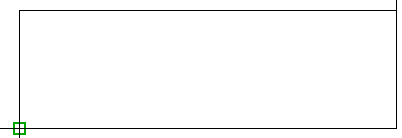
\includegraphics[scale=0.3]{pointdraw.png}}\hspace{20pt}
\subfloat[]{\label{fig:biaotilan1}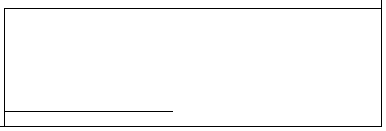
\includegraphics[scale=0.3]{biaotilan1.png}}\hspace{20pt}
\subfloat[]{\label{fig:biaotilan2}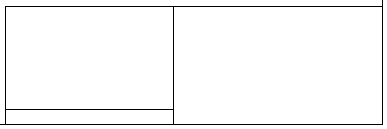
\includegraphics[scale=0.3]{biaotilan2.png}}
\caption{标题栏制作过程一}
\end{figure}
\begin{lstlisting}
命令: POINT
当前点模式:  PDMODE=0  PDSIZE=0.0000
指定点:
\end{lstlisting}
\item 绘制关键直线

以绘制的参考点为基础,绘制一条长80mm的水平线,结果如图\ref{fig:biaotilan1}所示。
\begin{lstlisting}
命令: LINE
指定第一个点: @0,7
指定下一点或 [放弃(U)]: @80,0
指定下一点或 [放弃(U)]:
\end{lstlisting}
以上一条直线的结束点为参考,分两段绘制一条56mm高的垂直线,结果如图\ref{fig:biaotilan2}所示。
\begin{lstlisting}
命令: LINE
指定第一个点: @0,-7
指定下一点或 [放弃(U)]: @0,28
指定下一点或 [放弃(U)]: @0,28
指定下一点或 [闭合(C)/放弃(U)]:
\end{lstlisting}

\begin{figure}[htbp]
\centering
\subfloat[]{\label{fig:biaotilan3.png}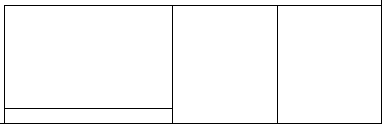
\includegraphics[scale=0.3]{biaotilan3.png}}\hspace{20pt}
\subfloat[]{\label{fig:biaotilan4.png}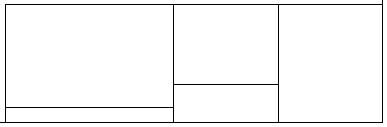
\includegraphics[scale=0.3]{biaotilan4.png}}\hspace{20pt}
\subfloat[]{\label{fig:biaotilan5.png}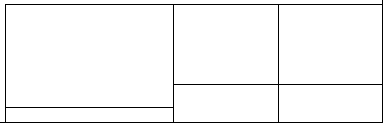
\includegraphics[scale=0.3]{biaotilan5.png}}
\caption{标题栏制作过程二}
\end{figure}

以上条重直线的结束点为参考,分四段绘制另一条垂直线,结果如图\ref{fig:biaotilan3.png}所示。
\begin{lstlisting}
命令: LINE
指定第一个点: @50,0
指定下一点或 [放弃(U)]: @0,-28
指定下一点或 [放弃(U)]: @0,-10
指定下一点或 [闭合(C)/放弃(U)]: @0,-9
指定下一点或 [闭合(C)/放弃(U)]: @0,-9
指定下一点或 [闭合(C)/放弃(U)]:
\end{lstlisting}
以上一条重直线的结束点为参考,绘制第二条水平线,结果如图\ref{fig:biaotilan4.png}所示。
\begin{lstlisting}
命令: LINE
指定第一个点: @0,18
指定下一点或 [放弃(U)]: @-50,0
指定下一点或 [放弃(U)]:
\end{lstlisting}
以第二条水平线的结束点为参考,绘制第三水平线,结果如图\ref{fig:biaotilan5.png}所示。
\begin{lstlisting}
命令: LINE
指定第一个点: @50,0
指定下一点或 [放弃(U)]: @50,0
指定下一点或 [放弃(U)]:
\end{lstlisting}
\item 绘制格线

完成关键直线的绘制后,可以应用AutoCAD的偏移命令来偏移产生标题栏表格格线。AutoCAD中调用偏移命令的方法有:
\begin{itemize}
\item 键盘输入OFFSET\index{offset,偏移}或O。
\item 【修改】$\rightarrow$【偏移】。
\item 【修改】$\triangleright$【偏移】图标
\includegraphics[scale=0.6]{offsettool.png}。
\end{itemize}
调用偏移命令后,会提示指定领衔距离,此时输入7并回车。
\begin{lstlisting}
命令: OFFSET
当前设置: 删除源=否  图层=源  OFFSETGAPTYPE=0
指定偏移距离或 [通过(T)/删除(E)/图层(L)] <通过>: 7
\end{lstlisting}
接下来命令提示选择要偏移的对象,此时按图\ref{fig:offsetselect.png}所示方式选择水平线作为偏移对象。
\begin{figure}[htbp]
\centering
\subfloat[]{\label{fig:offsetselect.png}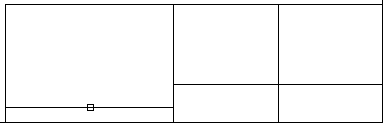
\includegraphics[scale=0.3]{offsetselect.png}}\hspace{20pt}
\subfloat[]{\label{fig:offsetselect1.png}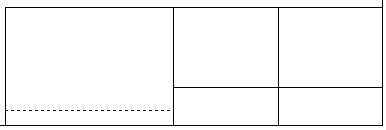
\includegraphics[scale=0.3]{offsetselect1.png}}\hspace{20pt}
\subfloat[]{\label{fig:offsetselect2.png}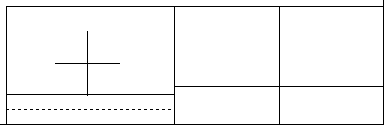
\includegraphics[scale=0.3]{offsetselect2.png}}
\caption{偏移操作过程}
\end{figure}
\begin{lstlisting}
选择要偏移的对象,或 [退出(E)/放弃(U)] <退出>:
\end{lstlisting}
选择完成后,会以图\ref{fig:offsetselect1.png}的虚线方式显示被选择的对象。接下来命令会提示指定要偏移的方向,此时将鼠移向虚线的上方,绘出现图\ref{fig:offsetselect2.png}所示的图线,单击鼠标左键即可完成偏移对象绘制。
接下来以继选择偏移对象,完成剩余的6条线的绘制,结果如图\ref{fig:offsetresult.png} 所示。
\begin{lstlisting}
指定要偏移的那一侧上的点,或 [退出(E)/多个(M)/放弃(U)] <退出>:
选择要偏移的对象,或 [退出(E)/放弃(U)] <退出>:
指定要偏移的那一侧上的点,或 [退出(E)/多个(M)/放弃(U)] <退出>:
选择要偏移的对象,或 [退出(E)/放弃(U)] <退出>:
指定要偏移的那一侧上的点,或 [退出(E)/多个(M)/放弃(U)] <退出>:
选择要偏移的对象,或 [退出(E)/放弃(U)] <退出>:
指定要偏移的那一侧上的点,或 [退出(E)/多个(M)/放弃(U)] <退出>:
选择要偏移的对象,或 [退出(E)/放弃(U)] <退出>:
指定要偏移的那一侧上的点,或 [退出(E)/多个(M)/放弃(U)] <退出>:
选择要偏移的对象,或 [退出(E)/放弃(U)] <退出>:
指定要偏移的那一侧上的点,或 [退出(E)/多个(M)/放弃(U)] <退出>:
选择要偏移的对象,或 [退出(E)/放弃(U)] <退出>:
\end{lstlisting}

\begin{figure}[htbp]
\centering
\subfloat[]{\label{fig:offsetresult.png}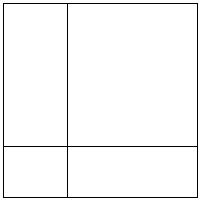
\includegraphics[scale=0.3]{offsetresult.png}}\hspace{30pt}
\subfloat[]{\label{fig:biaotilanresult1.png}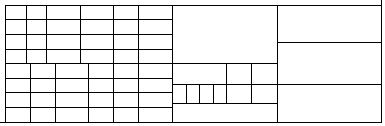
\includegraphics[scale=0.3]{biaotilanresult1.png}}
\caption{标题栏绘制过程三}
\end{figure}

接下来,重新启动命令并按照图\ref{fig:biaotilan}所示的尺寸,偏移产生其它的格线,整体的原则是切换一次,重新启动一次命令。最终结果如图\ref{fig:biaotilanresult1.png} 所示。
\item 设置文字样式

在标注文字以前需要根据国家标准设置文字样式。国家标准GB/T14691-1993规定:图样中的字体书写必须做到字体工整、笔画清楚、间隔均匀、排列整齐。字体高度(用$h$表示,单位mm)公称尺寸系列为:1.8,2.5,3.5,5,7,10,14,20。如果需要更大尺寸的字体,其字体高度应按$1:\sqrt{2}$的比率递增,用字体高度表示字号。汉字应写成长仿宋体字,并应采用中华人共和国国务院正式公布推行的《汉字简化方案》中规定的简化字。汉字高度$h$不应小于3.5mm,字的宽度一般为$\frac{h}{\sqrt{2}}$。数字和字母分为A型和B型。A型字体的笔画宽度为字高的$\frac{1}{14}$;B型字体的笔画宽度为字高的$\frac{1}{10}$。数字和字母均可写成直体或斜体,斜体字字关向右倾斜,与水平线成约$75^o$角。在一张图样上,只允许选用一种类型的字体。

在AutoCAD中调用文字样式设置命令的方式有:
\begin{itemize}
\item 键盘输入style\index{style,文字样式}或st
\item 【格式】$\rightarrow$【文字样式】
\item 【样式】
\includegraphics[scale=0.45]{styletools.png}工具栏中的【文字样式】
\includegraphics[scale=0.45]{textstyletool.png}图标
\end{itemize}

\begin{lstlisting}
命令:STYLE
\end{lstlisting}
命令调用后,会弹出图\ref{fig:textstyledialog.png}所示的文字样式对话框。此时,点击新建按钮,建立名称为“GB”的文字样式,然后将SHX字体设置为gbeitc.shx,大字体设置为gbcbig.shx,并“使用大字体”为选中状态,将“宽度因子”设置为0.76,点击应用按钮,使用GB文字样式置为当前,结果如图\ref{fig:textstyledialog2.png}所示。完成设置后,点击关闭按钮返回。
\begin{figure}[htbp]
\centering
\subfloat[]{\label{fig:textstyledialog.png}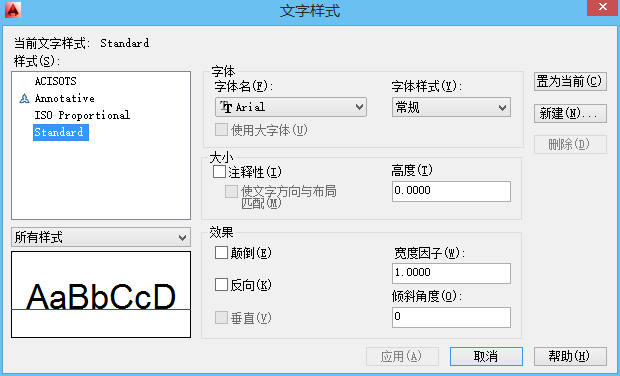
\includegraphics[scale=0.35]{textstyledialog.png}}\hspace{20pt}
\subfloat[]{\label{fig:textstyledialog2.png}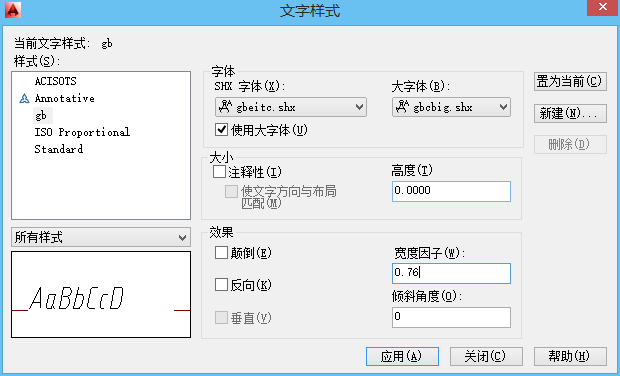
\includegraphics[scale=0.35]{textstyledialog2.png}}
\caption{文字样式设置}
\end{figure}
\item 标注文字

AutoCAD中标注文字需要用到文字命令,其调用方法有:
\begin{itemize}
\item 键盘输入MTEXT\index{mtext,多行文字}或MT
\item 【绘图】$\rightarrow$【文字】$\rightarrow$【多行文字】
\item 【绘图】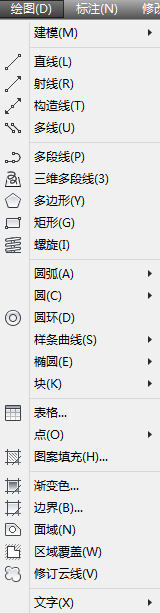
\includegraphics[scale=0.45]{drawtools.png}工具栏中【多行文字】
\includegraphics[scale=0.45]{texttool.png}图标
\end{itemize}

命令调用后,会提示指定第一角点,此时按图\ref{fig:textedit1.png}所示方式捕捉表格的倒数第一行的左上端点。
\begin{lstlisting}
命令: mtext
当前文字样式: "gb"  文字高度:  13.8924  注释性:  否
指定第一角点:
\end{lstlisting}
\begin{figure}[htbp]
\centering
\subfloat[]{\label{fig:textedit1.png}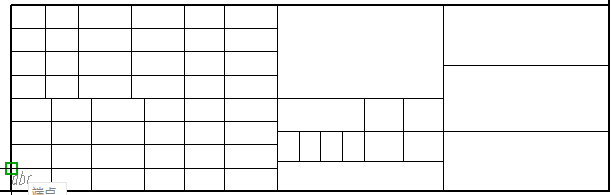
\includegraphics[scale=0.4]{textedit1.png}}\hspace{20pt}
\subfloat[]{\label{fig:textedit2.png}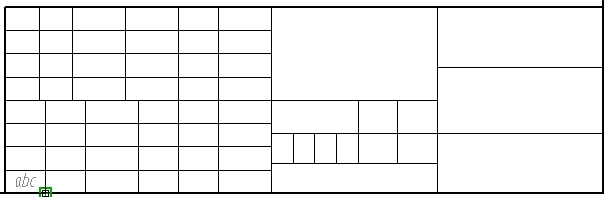
\includegraphics[scale=0.4]{textedit2.png}}
\caption{标注文字过程(一)}
\end{figure}
\begin{lstlisting}
指定对角点或 [高度(H)/对正(J)/行距(L)/旋转(R)/样式(S)/宽度(W)/栏(C)]: h
指定高度 <13.8924>: 5
\end{lstlisting}
完成第一角点指定后,提示指定对角点或选项,为使文字的字号符合国标的字高要求,因此输入【高度(H)】选项,并指定高度为5mm。
\begin{lstlisting}
指定对角点或 [高度(H)/对正(J)/行距(L)/旋转(R)/样式(S)/宽度(W)/栏(C)]: j
输入对正方式 [左上(TL)/中上(TC)/右上(TR)/左中(ML)/正中(MC)/右中(MR)/左下(BL)/中下(BC)/右下(BR)] <左上(TL)>: mc
\end{lstlisting}
完成文字高度设置后,为使文字能够位于表格的正中位置,故使用【对正(J)】选项,并选择【正中(MC)】位置。
\begin{lstlisting}
指定对角点或 [高度(H)/对正(J)/行距(L)/旋转(R)/样式(S)/宽度(W)/栏(C)]:
\end{lstlisting}
完成对正设置后,以图\ref{fig:textedit2.png}方式指定对角点,弹出图\ref{fig:textedit3.png}所示的文字输入对话框,并输入“工艺”后确定,结果如图\ref{fig:texteditresult1.png}所示。
\begin{figure}[htbp]
\centering
\subfloat[]{\label{fig:textedit3.png}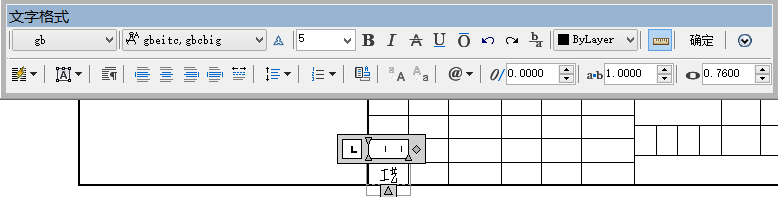
\includegraphics[scale=0.3]{textedit3.png}}\hspace{20pt}
\subfloat[]{\label{fig:texteditresult1.png}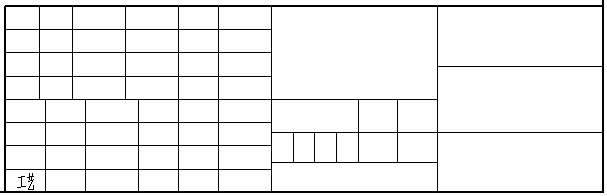
\includegraphics[scale=0.3]{texteditresult1.png}}
\caption{标注文字过程(二)}
\end{figure}

图\ref{fig:biaotilan}所示标题栏的其它文字的标注方式,与上述过程是一致的,其最终完成效果如图\ref{fig:texteditresult2.png}所示。
\begin{figure}[htbp]
\centering
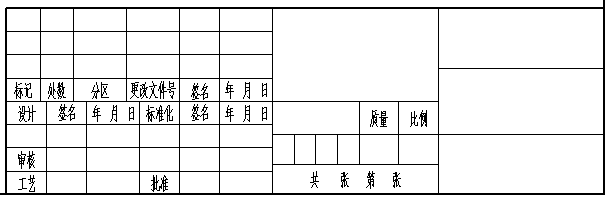
\includegraphics[scale=0.6]{texteditresult2.png}
\caption{标题栏结果}\label{fig:texteditresult2.png}
\end{figure}
\item 定制标题栏块

标题栏的图形和内容是基本固定的,并且每张图样都需要有标题栏。因此,应该把标题栏定义成一个组合体,以达到重重使用的目的。在AutoCAD中,实现这一要求的方式是定义块。所谓块是结合起来以创建单一对象的一个或多个对象。实现块定义的命令是创建块,其调用方法有:
\begin{itemize}
\item 键盘输入BLock\index{block,创建块}或B
\item 【绘图】$\rightarrow$【块】$\rightarrow$【创建】
\item 【绘图】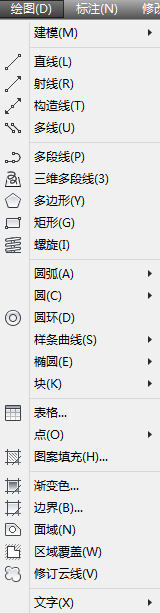
\includegraphics[scale=0.45]{drawtools.png}工具栏中【创建块】
\includegraphics[scale=0.45]{blocktool.png}图标
\end{itemize}
创建块命令调用后,会弹出图\ref{fig:blockcondection1.png} 所示的块定义对话框。此时在对话框的名称文本框中输入“GB标题栏”,点击
\includegraphics[scale=0.45]{selectpoint.png}图标,返回绘图区,以图\ref{fig:basepointselect.png} 所示的方式选择标题栏的右下角点做为基点,系统会自动获取选择点的坐标,若不指定则默认为坐标原点(0,0,0)点。然后,再点击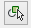
\includegraphics[scale=0.45]{blockobjselect.png}图标,以图\ref{fig:blockselect.png} 所示的方式选择整个标题栏做为定义块的对象,结果如图\ref{fig:blockset.png} 所示。完成操作后,点击确定即可完成块的定义。
\begin{figure}[htbp]
\centering
\subfloat[]{\label{fig:blockcondection1.png}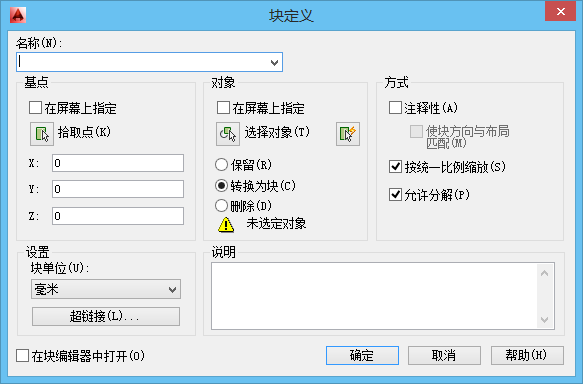
\includegraphics[scale=0.25]{blockcondection1.png}}\hspace{20pt}
\subfloat[]{\label{fig:basepointselect.png}\includegraphics[scale=0.4]{basepointselect.png}}\hspace{20pt}\\
\subfloat[]{\label{fig:blockselect.png}\includegraphics[scale=0.4]{blockselect.png}}\hspace{20pt}
\subfloat[]{\label{fig:blockset.png}\includegraphics[scale=0.25]{blockset.png}}
\caption{块定义过程}
\end{figure}
完成块定义后,只能实现文件内多次使用用,如果要实现与其它文件共享,需要有块写命令将块保存为文件,以便在其它文件中调入。调用块定命令的方式主要是用键盘输入WBLOCK\index{wblock,块写}或W。调用命令后,会弹出图\ref{fig:wblockdialog.png}所示的块写对话框。此时使块前的单选按钮处于选中状态,然后选择“GB标题栏”,最后选择适当的保存路径并点击确定,即可完成块写操作,实现文件间的共享。
\begin{figure}[htbp]
\centering
\includegraphics[scale=0.35]{wblockdialog.png}
\caption{块写对话框}\label{fig:wblockdialog.png}
\end{figure}
\end{procedure}
\subsection{标注尺寸}

连接杆零件图现在已经有了表达结构外形的视图,但是还不完整,主要是因为它还缺少表达零件大小的尺寸。一幅完整的图样不仅包括表达零件结构外形的视图,还需要标注确定零件大小的尺寸。由此可知,尺寸是图样的重要组成部分,其标注的正确、合理与否是影响图样质量的直接因素。为便于交流,国家标准GB/T4458.4-1984对尺寸进行了规定,要求在绘图过程中必须严格遵守。下面简要介绍一下与尺寸有关的规定和标注原则。

\subsubsection{尺寸的组成}
尺寸由尺寸界线、尺寸线和尺寸数字三部分组成。
\begin{enumerate}
\item 尺寸界线

尺寸界线用于表示所标注尺寸的起止范围,用细实绩绘制,并应该由图形的轮廓线、轴线或对称中心线引出。也可以直接利用轮廓线、轴线或对称中心线作为尺寸界线。尺寸界线应超出尺寸线$2\sim 5mm$。尺寸界线一般应与尺寸线垂直,必要时才允许倾斜。
\item 尺寸线

尺寸线用细实线绘制。标注线性尺寸时,尺寸线必须与所标注的线段平行,相同方向的各尺寸线之间的距离要均匀,间隔应大于$5mm$。尺寸线不能用图上的其它线代替,也不能与其他图线重合或在其延长线上,并应尽量避免与其他的尺寸线或尺寸界线交叉。尺寸线的终端有剪头和斜线两种形式。机械图样一般采用箭头形,只有在位置不够的情况下才允许用加圆点或斜线代替剪头。
\item 尺寸数字

线性数字一般注写在尺寸线的上方,也允许注写在尺寸线的中断处。其中$\phi $表示直径,$R$表示半径,$S$表示球面。
\end{enumerate} 

\subsubsection{尺寸标注的原则}
\begin{enumerate}
\item 图样中(包括技术要求和其它说明)的尺寸,以毫米为单位时,不需要标注计量单位的名称或符号;如采用其他单位,则必须注明相应的计量单位名称或符号;如$12m$、$45^o$等。
\item 图样上所标注的尺寸数值为实际物体的真实大小,与图形大小、比例及绘图的准确度无关。
\item 物体的第一个尺寸,在图样中一般只标注一次。
\item 图样中所标注的尺寸数值,为物体的最后完工尺寸,否则应另行注明。
\end{enumerate}
\begin{procedure}
\item 切换图层为“尺寸标注”图层
\item 设置标注样式

要应用AutoCAD标注符合国家标准的尺寸,首先需要根据国家标准的要求设置AutoCAD的尺寸标注样式。AutoCAD中调用尺寸标注样式命令的方式有:
\begin{itemize}
\item 键盘输入dimstyle\index{dimstyle,标注样式}或D
\item 【格式】$\rightarrow$【标注样式】
\item 【标注】$\rightarrow$【标注样式】
\item 【样式】\includegraphics[scale=0.45]{styletools.png}工具栏中的【标注样式】\includegraphics[scale=0.45]{dimstyletool.png}图标
\end{itemize}

\begin{lstlisting}
命令:dimstyle
\end{lstlisting}
命令调用后会弹出图\ref{fig:dimstyledialog.png} 所示的标注样式管理器,此对话框中列出了AutoCAD当前的所有样式、当前使用的样式及样式预览。为不改变AutoCAD的系统样式,我们需要新建与国标要求一致的标注样式。点击新建按钮弹出图\ref{fig:dimstylenew.png} 所示的新建标注样式对话框,选择ISO-25作为基础样式,并用于所用标注,建立名称为“GB标注样式”的新标注样式,完成后单击继续按钮,进入基础样式的设置。
\begin{figure}[htbp]
\centering
\begin{floatrow}[2]
\ffigbox{\caption{标注样式管理器}\label{fig:dimstyledialog.png}}{\includegraphics[scale=0.4]{dimstyledialog.png}}
\ffigbox{\caption{新建标注样式对话框}\label{fig:dimstylenew.png}}{\includegraphics[scale=0.7]{dimstylenew.png}}
\end{floatrow}
\end{figure}
\begin{enumerate}
\item 设置基础标注样式

\begin{figure}[htbp]
\centering
\subfloat[]{\label{fig:dimstylelineset.png}\includegraphics[scale=0.3]{dimstylelineset.png}}\hspace{20pt}
\subfloat[]{\label{fig:dimstylearrowset.png}\includegraphics[scale=0.3]{dimstylearrowset.png}}\\
\subfloat[]{\label{fig:dimstyletextset.png}\includegraphics[scale=0.3]{dimstyletextset.png}}\hspace{20pt}
\subfloat[]{\label{fig:dimstyledanweiset.png}\includegraphics[scale=0.3]{dimstyledanweiset.png}}
\caption{基础标注样式设置}
\end{figure}

\begin{itemize}
\item 设置线

完成基础样式名称设置后,会弹出样式设置对话框,并且“线”选项卡处于激活状态。此时,在线选项卡中,将尺寸线选项组中的基线间距设置为8;尺寸界线选项组中的超出尺寸线设置为2.5,起点偏移量设置为0。结果如图\ref{fig:dimstylelineset.png} 所示。

\item 设置符号和箭头

接下来设置符号和箭头选项卡,并按图\ref{fig:dimstylearrowset.png}所示结果,将箭头选项组中的引线设置为无,箭头大小设置为3.5;圆心标记选项组中的标记单选按钮置于选择状态,大小设置为2.5;弧长符号选项组设置为标注文字的上方。

\item 设置文字

接下来按图\ref{fig:dimstyletextset.png}所示设置文字选项卡,将文字外观选项组中的文字样式设置为GB,文字高度设置为5;文字位置选项组中的垂直设置为上,水平设置为居中,观察方向设置为从左到右,从尺寸线偏移设置为1.2;文字对齐设置为ISO标准。

\item 设置主单位

最后按图\ref{fig:dimstyledanweiset.png}所示设置主单位选项卡,将线性标注选项组中的精度设置为0.0000,小数分隔符设置为“.”句点,消零设置为后续;角度标注选项组精度设置为0.0,消零设置为后续。
\end{itemize}

设置完成后点击确定,返回标注样式管理器。基础标注样式设置完成后,标注样式还不能够达到国家标准的要求,还需要有针对性的设置基子样式。
\item 设置线性子标注样式

\begin{figure}[htbp]
\centering
\subfloat[]{\label{fig:subdimstylelinenew.png}\includegraphics[scale=0.55]{subdimstylelinenew.png}}\hspace{20pt}
\subfloat[]{\label{fig:subdimstylelineadjust.png}\includegraphics[scale=0.25]{subdimstylelineadjust.png}}
\caption{设置线性子标注样式}
\end{figure}

在标注样式管理器中,点击新建按钮弹出图\ref{fig:dimstylenew.png}所示的对话框,此时选择“GB标注样式”作为基础样式,并将用于“所有标注”修改为“线性标注”,结果如图\ref{fig:subdimstylelinenew.png} 所示,然后点击继续。

接下来按图\ref{fig:subdimstylelineadjust.png}所示设置调整选项卡,将文字位置设置为“尺寸线上方,带指引线”。设置完成后点击确定返回标注样式管理器。

\item 设置角度子标注样式

在标注样式管理器中,点击新新建按钮,按图\ref{fig:subdimstyleanglenew.png}所示选择“GB标注样式”作为基础样式,并将用于“所有标注”修改为“角度标注”,点击继续按钮进行子标注样式设置。

\begin{figure}[htbp]
\centering
\subfloat[]{\label{fig:subdimstyleanglenew.png}\includegraphics[scale=0.4]{subdimstyleanglenew.png}}\hspace{10pt}
\subfloat[]{\label{fig:subdimstyleangletextset.png}\includegraphics[scale=0.25]{subdimstyleangletextset.png}}\hspace{10pt}
\subfloat[]{\label{fig:subdimstyleangleadjustset.png}\includegraphics[scale=0.25]{subdimstyleangleadjustset.png}}
\caption{设置角度子标注样式}
\end{figure}

接下来按图\ref{fig:subdimstyleangletextset.png}所示设置角度子标注样式的文字设置,将文字对齐设置为水平。

最后按图\ref{fig:subdimstyleangleadjustset.png}所示设置角度子标注样式的调整设置,将文字位置设置为“尺寸线上方,带引线”,点击确定返回标注样式管理器。
\item 设置半径子标注样式

\begin{figure}[htbp]
\centering
\subfloat[]{\label{fig:subdimstylebanjinnew.png}\includegraphics[scale=0.55]{subdimstylebanjinnew.png}}\hspace{20pt}
\subfloat[]{\label{fig:subdimstylebanjinadjustset.png}\includegraphics[scale=0.25]{subdimstylebanjinadjustset.png}}
\caption{设置半径子标注样式}
\end{figure}

在标注样式管理器中,点击新新建按钮,按图\ref{fig:subdimstylebanjinnew.png}所示选择“GB标注样式”作为基础样式,并将用于“所有标注”修改为“半径标注”,点击继续按钮进行子标注样式设置。

按图\ref{fig:subdimstylebanjinadjustset.png}所示设置半径子标注样式的调整设置,将文字位置设置为“尺寸线旁边”,优化选项组中增加“手动放置文字”项,点击确定返回标注样式管理器。

\begin{figure}[htbp]
\centering
\subfloat[]{\label{fig:subdimstylezhijinnew.png}\includegraphics[scale=0.55]{subdimstylezhijinnew.png}}\hspace{20pt}
\subfloat[]{\label{fig:subdimstylezhijinadjustset.png}\includegraphics[scale=0.25]{subdimstylezhijinadjustset.png}}
\caption{设置直径子标注样式}
\end{figure}

\item 设置直径子标注样式

在标注样式管理器中,点击新新建按钮,按图\ref{fig:subdimstylezhijinnew.png}所示选择“GB标注样式”作为基础样式,并将用于“所有标注”修改为“半径标注”,点击继续按钮进行子标注样式设置。

按图\ref{fig:subdimstylezhijinadjustset.png}所示设置直径子标注样式的调整设置,将文字位置设置为“尺寸线旁边”,优化选项组中增加“手动放置文字”项,点击确定返回标注样式管理器。
\end{enumerate}

整个标注样式设置完成后,结果如图\ref{fig:dimstyleresult.png} 所示。要应用新建的“GB标注样式”,需要选中“GB标注样式”,并点击置为当前按钮。

当然也可以通过【样式】\includegraphics[scale=0.45]{styletools.png}工具栏中的标注样式控制列表框\includegraphics[scale=0.45]{dimstylelist.png}切换为“GB标注样式”\includegraphics[scale=0.45]{dimstylelist2.png}。

\begin{figure}[htbp]
\centering
\includegraphics[scale=0.45]{dimstyleresult.png}
\caption{新建标注样式结果}\label{fig:dimstyleresult.png}
\end{figure}
\item 标注尺寸

由于连接杆所要标注的尺寸都是线性尺寸,因此可以用AutoCAD的线性尺寸标注来完成,其主要的调用方法有:
\begin{itemize}
\item 键盘输入DIMLINEAR\index{dimlinear,线性标注}或dimlin
\item 【标注】$\rightarrow $【线性】
\item 【标注】\includegraphics[scale=0.45]{dimtoolsbar.png}工具栏中的【线性】\includegraphics[scale=0.45]{dimlinear.png}图标
\end{itemize}

\begin{figure}[htbp]
\centering
\subfloat[]{\label{fig:dimlinearfirstnode.png}\includegraphics[scale=0.4]{dimlinearfirstnode.png}}\hspace{10pt}
\subfloat[]{\label{fig:dimlinearsecondtnode.png}\includegraphics[scale=0.4]{dimlinearsecondtnode.png}}\hspace{10pt}
\subfloat[]{\label{fig:dimlinearpositionset.png}\includegraphics[scale=0.4]{dimlinearpositionset.png}}\hspace{10pt}
\subfloat[]{\label{fig:dimlinearresult.png}\includegraphics[scale=0.4]{dimlinearresult.png}}
\caption{线性标注过程}
\end{figure}

\begin{lstlisting}
命令: dimlinear
指定第一个尺寸界线原点或 <选择对象>:
\end{lstlisting}

线性标注命令调用后,按图\ref{fig:dimlinearfirstnode.png}所示指定端点作为第一个尺寸界线的原点。
\begin{lstlisting}
指定第二条尺寸界线原点:
\end{lstlisting}
接下来按图\ref{fig:dimlinearsecondtnode.png}所示,指定端点作为第二条尺寸界线的原点。
\begin{lstlisting}
指定尺寸线位置或
[多行文字(M)/文字(T)/角度(A)/水平(H)/垂直(V)/旋转(R)]:
标注文字 = 6
\end{lstlisting}
最后,按图\ref{fig:dimlinearpositionset.png}所示,用鼠标指定尺寸线的位置,即可完成一个线性尺寸的标。图\ref{fig:dimlinearresult.png}所示的结果为一水平线性尺寸。

通过观察可知,连接杆的水平尺寸是连续进行标注的,因此用AutoCAD的连续标注命令来完成更为简便快捷,其调用的方式有:
\begin{itemize}
\item 键盘输入dimcontinue\index{dimcontinue,连续标注}或dimcont
\item 【标注】$\rightarrow $【连续】
\item 【标注】\includegraphics[scale=0.45]{dimtoolsbar.png}工具栏中的【连续】\includegraphics[scale=0.45]{dimcontinue.png}图标
\end{itemize}
\begin{lstlisting}
命令: DIMCONTINUE
指定第二条尺寸界线原点或 [放弃(U)/选择(S)] <选择>:
标注文字 = 3
\end{lstlisting}
连续命令启动后,会自动以上次非连续标注尺寸的第二条尺寸界线的原点为起点,并提示指定第二条尺寸界线的原点,此时按图\ref{fig:dimcontinuesecondnode.png}所示指定第二条尺寸界线的原点,即可完成一线性尺寸的标注。

\begin{figure}[htbp]
\centering
\subfloat[]{\label{fig:dimcontinuesecondnode.png}\includegraphics[scale=0.6]{dimcontinuesecondnode.png}}\hspace{20pt}
\subfloat[]{\label{fig:dimcontinueresult.png}\includegraphics[scale=0.6]{dimcontinueresult.png}}
\caption{连续标注}
\end{figure}

接下来,可继续指定剩余的连续水平尺寸,结果如图\ref{fig:dimcontinueresult.png}所示。
\begin{lstlisting}
指定第二条尺寸界线原点或 [放弃(U)/选择(S)] <选择>:
标注文字 = 27
指定第二条尺寸界线原点或 [放弃(U)/选择(S)] <选择>:
标注文字 = 4
指定第二条尺寸界线原点或 [放弃(U)/选择(S)] <选择>:
标注文字 = 9
指定第二条尺寸界线原点或 [放弃(U)/选择(S)] <选择>:
选择连续标注:
\end{lstlisting}
至此,已经完成了所用的水平线性尺寸的标注。接下来的垂直方向的线性尺寸标与水平方向的线性尺寸标是基本相同的,唯一的区别是垂直方向的线性尺寸需要标注直径符号。
\begin{lstlisting}
命令: dimlinear
指定第一个尺寸界线原点或 <选择对象>:
指定第二条尺寸界线原点:
\end{lstlisting}
垂直线性尺寸标注指定尺寸界线原点的方式与水平线性尺寸的方式一致,当命令提示指定尺寸线位置或选项时,选择【多行文字(M)】项,在弹出的对话框中,点击符号\includegraphics[scale=0.4]{symbletool.png}列表,并选择直径符号即可完成直径形式文字的输入。
\begin{lstlisting}
指定尺寸线位置或
[多行文字(M)/文字(T)/角度(A)/水平(H)/垂直(V)/旋转(R)]: m
\end{lstlisting}
最后,用鼠标指定尺寸线的位置,即可完成重直线性尺寸的标注,结果如图\ref{fig:dimzhijinresult.png} 所示。
\begin{lstlisting}
指定尺寸线位置或
[多行文字(M)/文字(T)/角度(A)/水平(H)/垂直(V)/旋转(R)]:
标注文字 = 14
\end{lstlisting}

剩余的垂直线性尺寸标注过程与上述操作是一致的,因此不再重复,最终结果如图\ref{fig:dimresult.png} 所示。

\begin{figure}[htbp]
\centering
\subfloat[]{\label{fig:dimzhijinresult.png}\includegraphics[scale=0.6]{dimzhijinresult.png}}\hspace{20pt}
\subfloat[]{\label{fig:dimresult.png}\includegraphics[scale=0.6]{dimresult.png}}
\caption{垂直尺寸标注}
\end{figure}
\item 标注技术要求

由于连接杆的倒角尺寸未在图纸中予以标注,因此需要用文字在技术要求中注明未注倒角0.5的字样。此项操作可由多行文字命令完成。
\begin{lstlisting}
命令: MTEXT
当前文字样式: "gb"  文字高度:  5  注释性:  否
指定第一角点:
指定对角点或 [高度(H)/对正(J)/行距(L)/旋转(R)/样式(S)/宽度(W)/栏(C)]:
\end{lstlisting}
\end{procedure}

经过上述步骤的操作,最终完成的连接杆零件图如图\ref{fig:lianjieganbujuresult.png}所示。
\begin{figure}[htbp]
\centering
\includegraphics[scale=0.4]{lianjieganbujuresult.png}
\caption{连接杆布局结果}\label{fig:lianjieganbujuresult.png}
\end{figure}
\endinput